\chapter{Design of circuit}
  
  \section{DC Bias point}

  We are using ADS to simulate the I-V characteristics of the CGH40010 transistor. ADS is providing a built-in design guide for this purpose. Figure~\ref{fig:fig_IV} shows the I-V characteristics, with drain current on the y-axis, drain voltage on the x-axis and curves for various gate voltages from -5 to -1 volts in 0.2 volts increments. Refering to figure 5.12 in \cite[p.~200]{AmpRobertson}, we choose to set a bias point at approximately 70\% of the maximum saturated drain current IDS, to achieve a compromise between good linearity and high gain. We find this to be a gate voltage of about -1 volts.

  \begin{figure}[h]
	  \label{fig:fig_IV}
	  \centering
	  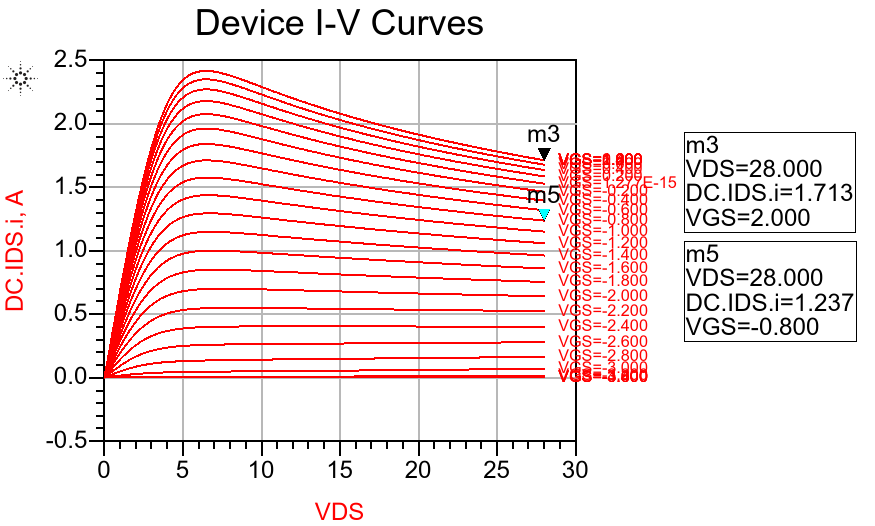
\includegraphics[width=0.75\textwidth]{img/01_IVCurve.png}
	  \caption{I-V curve characteristics for CGH40010}
  \end{figure}

  \section{Bias network}

  \section{Power supply filtering}

  \section{Matching network}
